\chapter{Projeto e Implementação}
Neste capítulo, entraremos em mais detalhes da parte de projeto e implementação do sistema, com base nos requisitos já levantados, passando pelas tecnologias envolvidas e pela arquitetura do sistema.

\section{Elaboração e Estrutura do Sistema}
Está seção explica, com mais detalhes, os casos de uso do sistema, as responsabilidades em comum entre cada um deles e como isso pode ser estruturado na arquitetura.

\subsection{Casos de Uso}
Com bases nos requisitos levantados anteriormente, foram construídos os casos de uso a seguir (para mais detalhes, ver o apêndice \href{chap:use-case-appendix}):

\begin{itemize}
    \item Propor tema de trabalho
    \item Login
    \item Cadastrar disciplinas
    \item Editar disciplinas
    \item Cadastrar grupos de trabalhos
    \item Cadastrar professores
    \item Cadastrar pessoas externas
    \item Entregar atividade
    \item Listar entregas
    \item Listar necessidades adicionais
    \item Construir bancas práticas
    \item Construir bancas teóricas
    \item Avaliar projetos práticos
    \item Avaliar monografias teóricas
    \item Calcular nota final dos projetos
    \item Importar projetos aprovados
    \item Cadastrar projetos avulsos
    \item Buscar projetos anteriores
    \item Buscar temas propostos
\end{itemize}

\subsection{Diagramas de Casos de Uso}
Os casos de uso foram estruturados nos seguintes diagramas (elaborados com a ajuda da ferramenta PlantText \cite{planttext2018}, para ver como elas foram geradas, ver apêndice \href{chap:use-case-appendix}):

\begin{figure}[H]
    \centering
    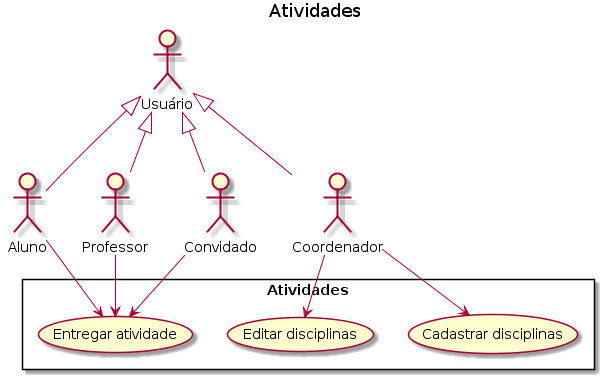
\includegraphics[scale=0.6]{atv.png}
    \caption{Diagrama de Casos de Uso para Atividades}
    \label{fig:use-case-atv}
\end{figure}

\begin{figure}[H]
    \centering
    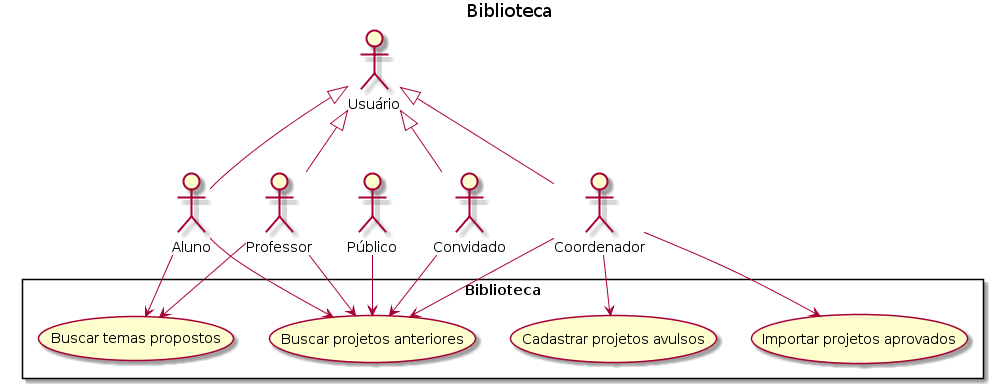
\includegraphics[scale=0.4]{bib.png}
    \caption{Diagrama de Casos de Uso para Base de Dados (Biblioteca Virtual)}
    \label{fig:use-case-atv}
\end{figure}

\begin{figure}[H]
    \centering
    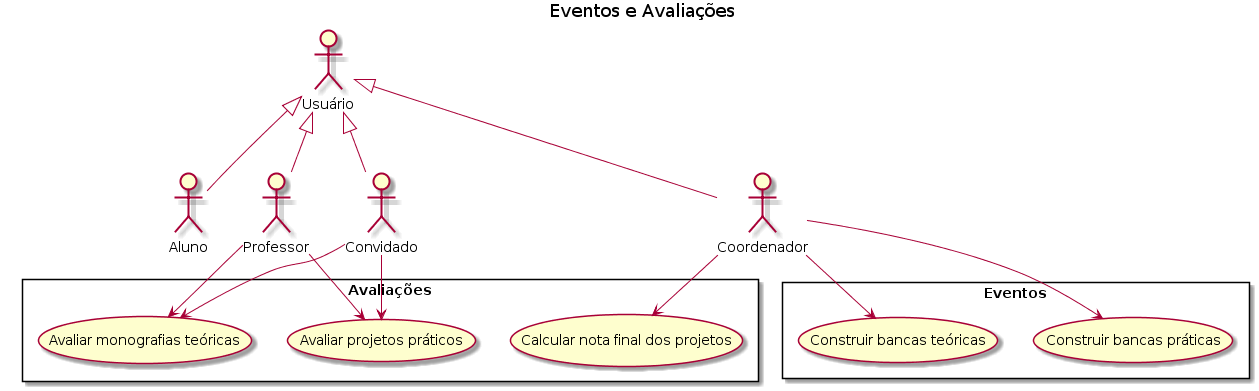
\includegraphics[scale=0.3]{ev-ava.png}
    \caption{Diagrama de Casos de Uso para Eventos e Avaliações}
    \label{fig:use-case-atv}
\end{figure}

\begin{figure}[H]
    \centering
    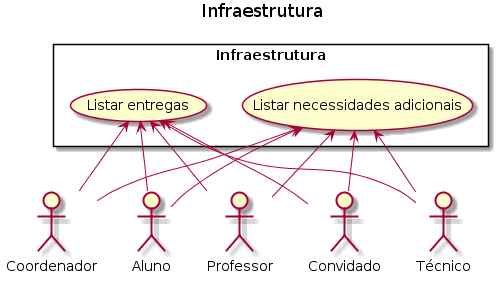
\includegraphics[scale=0.6]{infra.png}
    \caption{Diagrama de Casos de Uso para Infraestrutura}
    \label{fig:use-case-atv}
\end{figure}

\begin{figure}[H]
    \centering
    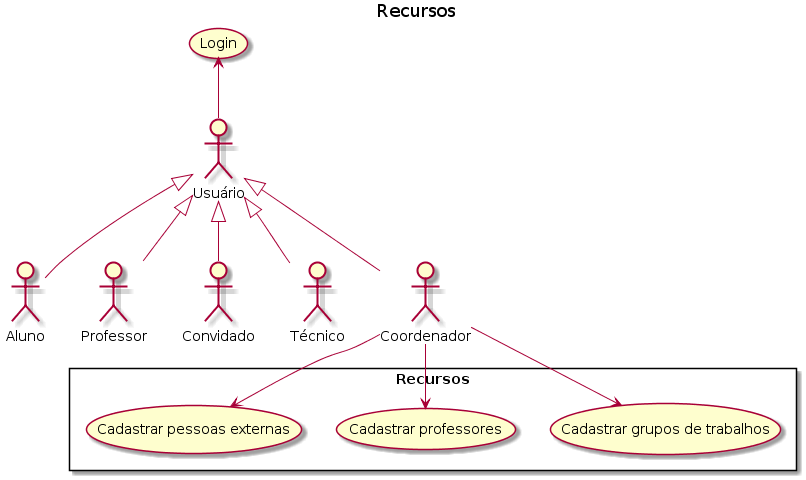
\includegraphics[scale=0.5]{recursos.png}
    \caption{Diagrama de Casos de Uso para Gerenciamento dos Recursos}
    \label{fig:use-case-atv}
\end{figure}

\section{Tecnologias Utilizadas}
Após determinar os requisitos do sistema e estabelecer os casos de uso, resta determinar as tecnologias a serem usadas, bem como a arquitetura do sistema.

Como parte dos requisitos, era necessário o uso de sistemas \textit{web} para os \textit{stakeholders} terem maior mobilidade e facilidade ao realizarem as interações com o sistema. Sendo assim, é valido passar por alguns conceitos tecnológicos do projeto.

\subsection{\textit{Frameworks web} e o Django}
É comum, em desenvolvimento de sistemas, usar soluções prontas como forma de simplificar o desenvolvimento de soluções. Essas soluções são conhecidas como arcabouços (ou \textit{frameworks})\cite{iansommerville2011}: "Um framework é uma estrutura genérica estendida para se criar uma aplicação ou subsistema mais específico.". Para este projeto, foi usado um \textit{framework}, em linguagem Python, chamado \textbf{Django}.

O Django é estruturado em aplicações (apps), onde cada aplicação corresponde a uma parte do sistema, geralmente independente e reciclável (ou seja, pode ser usada em aplicações Django diferentes). Cada aplicação segue o padrão \textit{Model-View-Controller}.

O padrão \textit{Model-View-Controller} - MVC é um padrão arquitetural para organizar os componentes da aplicação. Ele é dividido em três grandes grupos\cite{thedjangobook2018}:

\begin{itemize}
    \item Modelo (\textit{Model}): Uma representação (interface) para os dados da aplicação.
    \item Visualização (\textit{View}): Camada de apresentação dos dados da aplicação. No caso do Django, ele é chamado de \textit{Template}.
    \item Controlador (\textit{Controller}): Camada de controle que interliga o modelo com a apresentação dos dados, onde geralmente fica a lógica de negócio. No caso do Django, ele é conhecido como \textit{View}.
\end{itemize}

A vantagem do padrão está no fluxo de dados que existe entre os grupos, além de evitar códigos com funcionalidades diferentes em lugares errados, como, por exemplo, lógica de negócio na camada de apresentação.

\subsection{Arquitetura}
O Django foi usado na versão mais recente estável (2.1), que corrigiu algumas novidades da versão 2.0. É esta versão que foi usada pelo projeto em questão, dado que é estável e possui suporte de apoio da equipe até Dezembro de 2020\cite{djangodownload}. Ele usa, como padrão, o SQLite, o que atendeu bem durante o desenvolvimento. Já o Heroku tem como banco de dados padrão o PostgreSQL, o que exigiu o chaveamento entre os bancos no ambiente local de desenvolvimento e os ambientes de validação hospedados no serviço. Por isso, o projeto possui configurado dois pacotes de gerenciamento de banco de dados, um para SQLite (nativo do Django), outro para PostgreSQL (o Psycopg\cite{lucassouto2017}).

Para controlar os acessos ao sistema, por limitações do Django, cada pessoa terá um único usuário, com vários perfis diferentes de acesso, cada qual com suas permissões e ações. São quatro perfis diferentes de acesso: estudante, docente, convidado e coordenador. Cada usuário pode ter um ou mais perfis de acesso simultâneos (é o caso, por exemplo, dos coordenadores da disciplina, que também são docentes e podem orientar e avaliar projetos).

\subsection{Aplicações Construídas}
O sistema foi estruturado em aplicações menores \textit{apps}, cada uma com uma responsabilidade:

\begin{itemize}
    \item home: Aplicação responsável por gerenciar as funções básicas a todos os usuários, como por exemplo login/logout, o conteúdo da página de entrada, entre outros.
    \item users: Gerencia os usuários cadastrados do sistema e os seus perfis (aluno, docente, convidado e coordenador)
    \item disciplines: Gerencia as disciplinas de TCC do curso, duas disciplinas por ano (TCC1 e TCC2).
    \item activities: Gerencia as atividades das diversas disciplinas do sistema.
    \item workgroups: Cuida dos grupos de trabalho criados durante as disciplinas. 
    \item deliveries: Cuida das entregas das atividades do curso, cada uma realizada pelos grupos de trabalho e revisadas pelos orientadores/co-orientadores.
    \item rooms: Cuida das salas que serão usadas nos eventos de bancas teóricas e práticas.
    \item events: Gerencia os eventos teóricos e práticos que ocorrem nas disciplinas de TCC2.
    \item allocations: Cuida das alocações de cada grupo, para cada evento teórico ou prático, junto com os convidados e docentes que avaliarão o grupo.
    \item evaluations: Gerencia as avaliações que cada docente ou convidado alocado fará nos eventos.
    \item rules: Determina as disciplinas e os eventos que serão usados para calcular as notas finais.
    \item score: Gerencia as notas finais calculadas para cada situação, por grupo de trabalho.
\end{itemize}